\documentclass{ximera}


\graphicspath{
  {./}
  {ximeraTutorial/}
  {basicPhilosophy/}
}

\newcommand{\mooculus}{\textsf{\textbf{MOOC}\textnormal{\textsf{ULUS}}}}


\usepackage{tkz-euclide}\usepackage{tikz}
\usepackage{tikz-cd}
\usetikzlibrary{arrows}
\tikzset{>=stealth,commutative diagrams/.cd,
  arrow style=tikz,diagrams={>=stealth}} %% cool arrow head
\tikzset{shorten <>/.style={ shorten >=#1, shorten <=#1 } } %% allows shorter vectors

\usetikzlibrary{backgrounds} %% for boxes around graphs
\usetikzlibrary{shapes,positioning}  %% Clouds and stars
\usetikzlibrary{matrix} %% for matrix
\usepgfplotslibrary{polar} %% for polar plots
\usepgfplotslibrary{fillbetween} %% to shade area between curves in TikZ
\usetkzobj{all}
\usepackage[makeroom]{cancel} %% for strike outs
%\usepackage{mathtools} %% for pretty underbrace % Breaks Ximera
%\usepackage{multicol}
\usepackage{pgffor} %% required for integral for loops



%% http://tex.stackexchange.com/questions/66490/drawing-a-tikz-arc-specifying-the-center
%% Draws beach ball
\tikzset{pics/carc/.style args={#1:#2:#3}{code={\draw[pic actions] (#1:#3) arc(#1:#2:#3);}}}



\usepackage{array}
\setlength{\extrarowheight}{+.1cm}
\newdimen\digitwidth
\settowidth\digitwidth{9}
\def\divrule#1#2{
\noalign{\moveright#1\digitwidth
\vbox{\hrule width#2\digitwidth}}}
























%%This is to help with formatting on future title pages.
\newenvironment{sectionOutcomes}{}{}


\author{Jim Talamo and Bart Snapp}
\license{Creative Commons 3.0 By-NC}


\outcome{Compute integrals involving powers of sine and cosine}
\outcome{Recognize the patterns that appear in trigonometric integrals,
  and use appropriate substitutions to compute them.}


\begin{document}
\begin{exercise}

This exercise explores a general method of integrating products of $\sin(x)$ and $\cos(x)$ when the power of $\sin(x)$ is odd.  For any odd integer, we can find an integer $k$ so that the original odd integer takes the form $2k+1$.  For instance:

\begin{exercise}
If our original odd integer is $7$, we can express $7 = 2 \cdot \answer{3}+1$, so $k=\answer{3}$.

If our original odd integer is $93$, we can express $93 = 2 \cdot \answer{41}+1$, so $k=\answer{41}$.
\end{exercise}

 If we are integrating a product of powers of sine and cosine functions, and the power of sine is odd, then the integral looks like
\[
\int \sin^{2k+1}(x) \cos^m(x) dx
\]
where $k$ and $m$ are integers.  Then:

\begin{align*}
  \int \sin^{2k+1}(x) \cos^m(x) dx &=\int(\sin^{2}(x))^2 \cos^m(x) \sin(x) dx\\
  &= \int (1-\cos^2(x))^2 \cos^m(x) \sin(x)dx.
\end{align*}
We have now set ourselves up for an eventual substitution:
\begin{center}%% used center instead of image since there is no reason for a LARGE integral in the text
  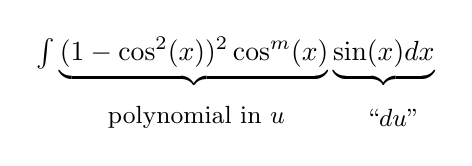
\begin{tikzpicture}
    \node at (0,0) {
      $\int \underbrace{(1-\cos^2(x))^2 \cos^m(x)} \underbrace{\sin(x) dx}$
        };
    \node at (-.5,-.7) {\small{polynomial in $u$}};
    \node at (2,-.7) {\small{``$du$''}};
  \end{tikzpicture}
\end{center}
so letting $u = \cos(x)$ so $du =\answer{-\sin(x)} dx$, we have
\[
  \int \sin^{2k+1}(x) \cos^m(x) dx =\int(\sin^{2}(x))^2 \cos^m(x) \sin(x) dx = \int -(1-u^2)^2 u^m du
\]
which is a polynomial, and can be integrated term-by-term after expansion.

Of course, this was quite general, and a real example is worth a thousand generalities:

\begin{exercise}
We find $\int \sin^5(x) \cos^4(x) dx$ by following the above prototype.  Here we have:

\[
\int \sin^{2k+1}(x) \cos^m(x) dx
\]
and can find that $k=\answer{2}$ and $m=\answer{4}$.

\begin{align*}
  \int \sin^{2k+1}(x) \cos^4(x) dx &=  \int \sin^{2(2)+1}(x) \cos^4(x) dx \\
  &= \int(\sin^{2}(x))^2 \cos^4(x) \sin(x) dx\\
  &= \int (1-\cos^2(x))^2 \cos^4(x) \sin(x)dx.
\end{align*}
We have now set ourselves up for an eventual substitution:
\begin{center}%% used center instead of image since there is no reason for a LARGE integral in the text
  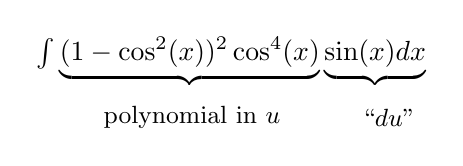
\begin{tikzpicture}
    \node at (0,0) {
      $\int \underbrace{(1-\cos^2(x))^2 \cos^4(x)} \underbrace{\sin(x) dx}$
        };
    \node at (-.5,-.7) {\small{polynomial in $u$}};
    \node at (2,-.7) {\small{``$du$''}};
  \end{tikzpicture}
\end{center}
so letting $u = \cos(x)$ so $du =\answer{-\sin(x)} dx$, we have
\[
\int -(1-u^2)^2 u^4 du
\]
which is a polynomial, and can be integrated term-by-term after expansion.  

\begin{exercise}
We can now perform this expansion since we have actual constants to find:

\[  \int(\sin^{2}(x))^2 \cos^4(x) \sin(x) dx = \int -u^8+2u^6-u^4 du =\answer{-\frac{1}{9}u^9+\frac{2}{7}u^7-\frac{1}{5}u^5 +C}\]

(Use $C$ for the constant of integration and express your antiderivative in terms of $u$)
\begin{exercise}

Reversing the substitution gives:

\[
\int \sin^5(x) \cos^4(x) dx=\answer{-\frac{1}{9}\sin^9(x)+\frac{2}{7}\sin^7(x)-\frac{1}{5}\sin^5(x) +C}
\]
\end{exercise}


\end{exercise}
\end{exercise}
\end{exercise}
\end{document}
